% Chapter Template

\chapter{ESTABLISHMENT OF EXPERIMENTATION PLATFORM} % Main chapter title

\label{Chapter5} % Change X to a consecutive number; for referencing this chapter elsewhere, use \ref{ChapterX}

\lhead{Chapter 5. \emph{ESTABLISHMENT OF EXPERIMENTATION PLATFORM}} % Change X to a consecutive number; this is for the header on each page - perhaps a shortened title

As the state-of-the-are about VMI is finished and the objective is determined, we plan to implement a prototype in
KVM virtualization platform. With a HP workstation at disposal, we need firstly to establish an experimentation and
development platform.

%----------------------------------------------------------------------------------------
%	SECTION 1
%----------------------------------------------------------------------------------------

\section{WIN7 and UBUNTU DUAL-BOOT SYSTEM}

As was mentioned above, the first step to achieve our final objective is to figure out how derivative pattern functions by
installing and manipulating the only known open-source derivative pattern VMI application: Nitro. Thus, it’s logical to
choose those operating systems which support Nitro. According to Pfoh, Nitro has been tested on Linux kernel 3.11 and
3.13. Hence, Ubuntu14.04 with kernel version 3.13 is our final choice. KVM virtualization platform will be built in a HP Z820 workstation 
which initially has only Windows 7 installed. The first step is to install a Windows 7 and Ubuntu 14.04 dual-boot system. This manipulation
is not difficult but kind of tedious. In fact, we follow this tutorial http://askubuntu.com/questions/343268/how-to-use-manual-partitioning-during-
installation to accomplish this step.

%-----------------------------------
%	SUBSECTION 2
%-----------------------------------

\section{NETWORK CONFIGURATION}

This workstation has been allocated a static network configuration and it uses always port 8 in each office. To achieve
this, we need to edit configuration file /etc/network/interfaces to set 10.193.192.37 as ipv4 address, 255.255.255.0 as
10network mask, 10.193.192.1 as default gateway and 10.193.197.10 as DNS name server. The final network configuration in 
Ubuntu14.04 is shown as in Figure \ref{fig:HP Workstation static network configuration}.

\begin{figure}[htbp]
	\centering
		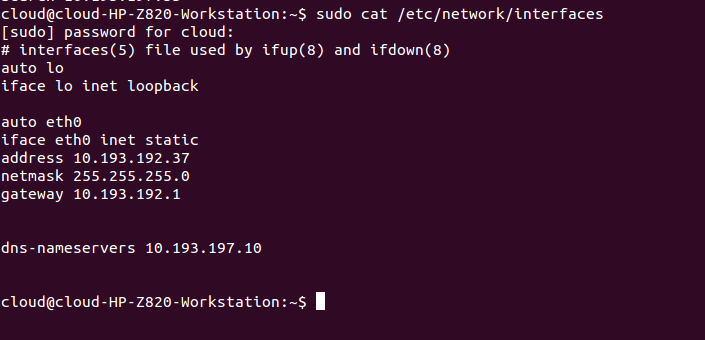
\includegraphics[scale = 0.8]{Figures/Figure5.png}
	\caption[HP Workstation static network configuration]{HP Workstation static network configuration}
	\label{fig:HP Workstation static network configuration}
\end{figure}

Besides, never forget to set a parameter named “managed” to “true”, defined in configuration file /etc/NetworkManager/NetworkManager.conf. 
Otherwise the network will be always in disable state. The security politics of Orange Labs require each PC to configure proxy server if the 
former needs Internet connectivity. In fact, under Linux system, it is possible to set proxy configuration on different level. The first 
solution is to declare http proxy server on command-line level. For example, if we want to update APT source list, we could issue a command in 
a terminal:
\shellcmd{sudo http://proxy.rd.francetelecom.fr:8080 apt-get update}
This proxy configuration is uniquely valid for the current command and every command we tape should contain an option for proxy server, which is
not effective and tedious. Proxy server configuration could also be set on application level. For example, if we want to user web browser such 
as Firefox, we need to set proxy address for Firefox just like in the following picture.

\begin{figure}[htbp]
	\centering
		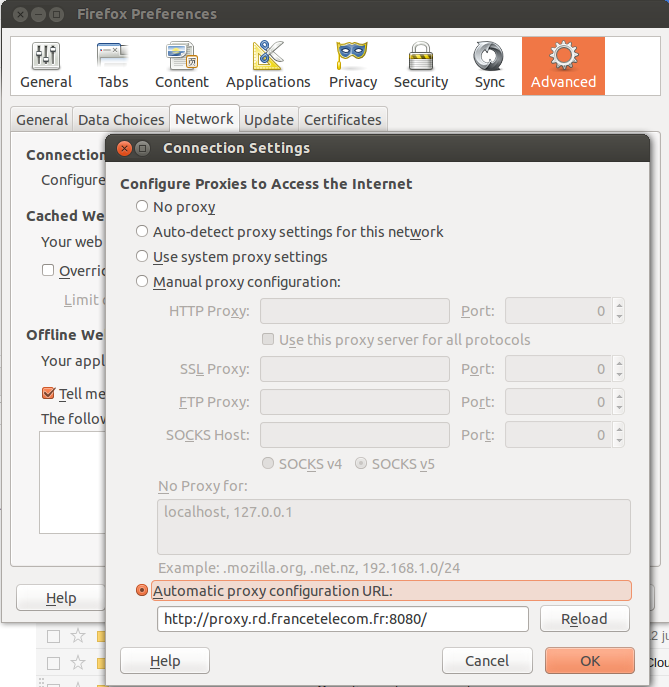
\includegraphics[width=12cm, height= 9cm ]{Figures/Figure6.png}
	\caption[Firefox proxy parameter]{Firefox proxy parameter}
	\label{fig:Firefox proxy parameter}
\end{figure}

To use APT command to install software, we need to edit (if not exist, create) a configure file named \lq apt.conf \rq under /etc/apt. This file just contains one line: Acquire::http::proxy::”http://proxy.rd.francetelecom.fr:8080”
Then we could issue command like \lq sudo apt-get install software\_name \lq as normal in terminal. In one word, it is supposed to configure proxy server address for every application which needs Internet connectivity.
The last solution is setting bash configuration files like /etc/profile, /etc/bash.bashrc or ~/.bashrc. Proxy configuration in this manner is user or all-user level. Only once configuration is needed to guarantee Internet connectivity for all applications.


%----------------------------------------------------------------------------------------
%	SECTION 3
%----------------------------------------------------------------------------------------
\section{KVM Introduction}

After installation of Ubuntu14.04 in our workstation, it’s time to install required Ubuntu packages to turn Ubuntu into a hypervisor. Prior to the real installation, it is necessary to make a presentation for KVM.

KVM (Kernel-based Virtual Machine) is a virtualization infrastructure for the Linux kernel that turns it into a hypervisor, which was merged into the Linux kernel mainline in February 2007. KVM requires a processor with hardware virtualization extension. KVM has also been ported to FreeBSD and Illumos in the form of loadable kernel modules. 
Compared to other virtualization alternatives available in Linux, KVM presents the following advantages \cite{Reference20}:

    \begin{itemize}
	\item Can interact directly with the Kernel
	\item Default virtualization in leading Linux Distributions
	\item One of the Linux software developed aggressively.
	\item Almost becoming competitor to VMware by implementing technologies such as v2v, p2v, and many open source tools to manage VM
	\item Number of open source cloud automation softwares use KVM as default hypervisor 
    \end{itemize}

%----------------------------------------------------------------------------------------
%	SECTION 4
%----------------------------------------------------------------------------------------

\section{KVM’s Operating Principle \cite{Reference20}}

Once KVM is installed on a Linux box, a hardware file /dev/kvm is created which will act as interpreter between actual hardware and hypervisor 
manager (for example, virt-manager). Whenever a request for hardware changes or additions comes from hypervisor manager, KVM software starts 
allocating those resources virtually by interacting with real hardware. Suppose we want to change RAM on a virtual machine, this is communicated
by the hypervisor manager to KVM for allocating the resource. Then KVM interacts with hardware and reserves that RAM from real RAM for that particular VM. This happens for the other resources as well.

\begin{figure}[htbp]
	\centering
		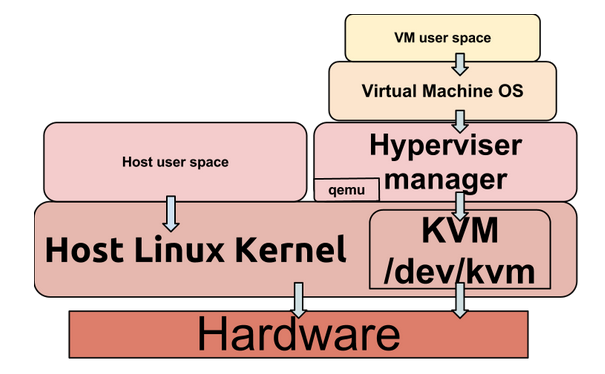
\includegraphics[scale = 0.6]{Figures/Figure7.png}
	\caption[KVM Virtualization Architecture in Linux]{KVM Virtualization Architecture in Linux \cite{Reference20}}
	\label{fig:KVM Virtualization Architecture in Linux}
\end{figure}


\section{KVM’s VM Management Tools}

There exists several methods in KVM for management activity such as guest’s creation, deletion, start, stop and clone,etc.

\subsection{virt-manager}
The most popular GUI is called Virtual Machine Manager (VMM), developed by RedHat. 
The tool is also known by its generic package name virt-manager. 
It comes with a number of supporting tools, including virt-install, virt-clone, virt-image, and virt-viewer, 
which are used to provision, clone, install, and view virtual machines, respectively. 
VMM also supports Xen machines. Virt-manager relies on libvirt and uses qemu to run guest instance. 
In the following section, we will show how to create a KVM guest with virt-manager.

\subsection{virsh}
The generic KVM command interface is provided by virsh. virsh is a shell for managing hypervisors and VM’s directly from host OS terminal. 
Specifically, you can use the supporting tools, like virt-install for creating your virtual machines. 
On Ubuntu, there's a special ubuntu-vm-builder tool that can be used for provisioning Ubuntu builds, developed by Canonical.

\subsection{qemu command line with ''enable-kvm'' option}
In fact, virt-manager or virsh both could be regarded as wrapper based on libvirt and qemu. 
As a result, we could use qemu command lines to manage KVM guests with “enable-kvm” option to profit performance acceleration offered by KVM. 
However, this method is not handy compared to virt-manager and virsh. 
Note that Nitro is only able to monitor KVM guests launched by a modified version qemu. 
We could use GUI tools such as virt-manager to create virtual machines images and issue qemu command line to start created VM and start Nitro to monitor these VMs.

\subsection{KVM command}
KVM also has its own syntax, similar to QEMU. 
It is not a recommended way of managing virtual machines. 
More information is available with link: https://help.ubuntu.com/community/KVM/Directly

\subsection{Libvirt}
Libvirt is not a VM management tool. Instead, it is a toolkit to interact with the virtualization capabilities of recent versions of Linux 
\cite{Reference23}. It is an open-source project and provides a set of long term stable C API. These C APIs all APIs are designed to do 
virtualization management, such as: provision, create, modify, monitor, control, migrate and stop the guests - within the limits of the support
of the hypervisor for those operations. Hence, libvirt is intended to be a building block for higher level management tools and for applications
focusing on virtualization of a single physical host. The Figure \ref{fig:Relationship between virsh, virt-manager and libvirt} shows the 
relationship between hypervisor, libvirt and virtualization management tool.

\begin{figure}[htbp]
	\centering
		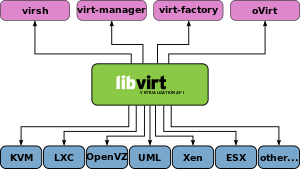
\includegraphics[scale = 1.2]{Figures/Figure8.png}
	\caption[Relationship between virsh, virt-manager and libvirt]{Relationship between virsh, virt-manager and libvirt \cite{Reference25}}
	\label{fig:Relationship between virsh, virt-manager and libvirt}
\end{figure}

\section{KVM/QEMU networking}
Guest (VM) networking in KVM is the same as in qemu, 
so it is possible to refer to other documentations about networking for qemu. 
In this section, we will talk about the three most frequent types of network needed.
\subsection{User Networking}
This networking mode, shown in figure \ref{fig:User networking mode topology}, allows guests accessing to the host, to the internet. 
However, the guests are neither invisible from outside network nor from other VMs. 
In addition, user networking does not support other network protocols other than TCP/UDP. 
Hence, certain applications (like ping) won't work.

\begin{figure}[htb]
	\centering
		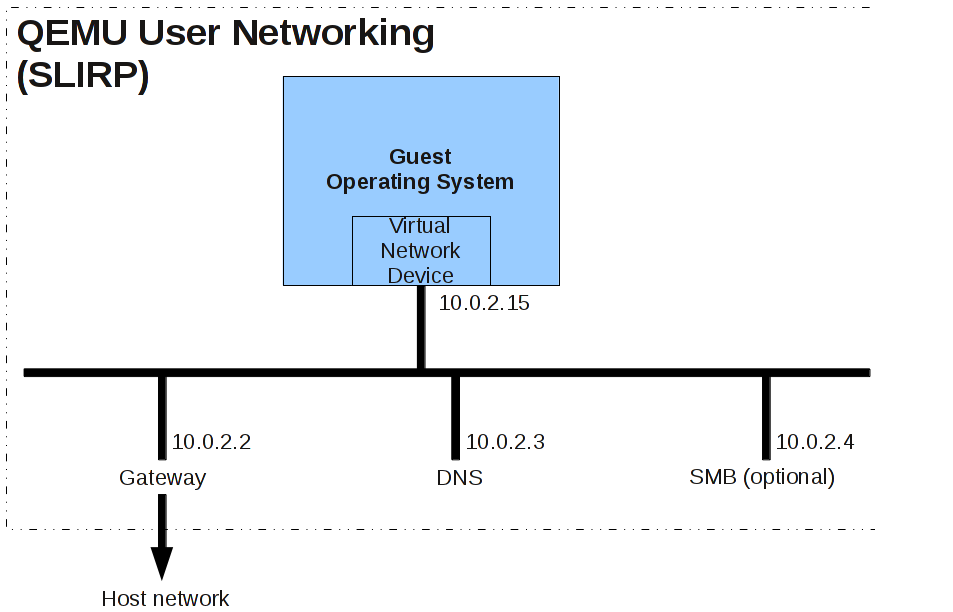
\includegraphics[scale=0.5]{Figures/Figure9.png}
	\caption[User networking mode topology]{User networking mode topology \cite{Reference24}}
	\label{fig:User networking mode topology}
\end{figure}

For example, we could issue the following to start a guest in user networking mode:
\shellcmd{qemu-system-x86\_64 -enable-kvm -had win7.img -m 2048}
The guest OS will see an E1000 NIC with a virtual DHCP server on 10.0.2.2 and will be 
allocated an address starting from 10.0.2.15. A virtual DNS server will be accessible on 10.0.2.3.

\subsection{Bridged Networking}
The bridge networking mode makes all launched guests run just like they are in the same local network with host machine.  
To use bridged networking, a virtual Ethernet bridge should be firstly created. Under Ubunu14.04, 
we need to edit /etc/network/interfaces as following, for example:

\# The content of file /etc/network/interfaces\\
\# Replace old eth0 config with br0, there no more "auto eth0" \\
auto br0\\
\# Use old eth0 config for br0, plus bridge stuff\\
iface br0 inet static\\
	\indent\indent \# Attention use old static configuration of eth0\\
	\indent\indent bridge\_ports    eth0\\
	\indent\indent bridge\_stp      off\\
	\indent\indent bridge\_maxwait  0\\
	\indent\indent bridge\_fd       0\\
	
Run each guest with the following, replacing \$macaddress with a customized MAC address.
\shellcmd{qemu-system-x86\_64 -hda /path/to/hda.img -device e1000,netdev=net0,mac=\$macaddress-netdev tap,id=net0}

\subsection{networking mode}
NAT networking mode is actually the default networking mode for virtual machines created by virt-manager.
\begin{figure}[htb]
	\centering
		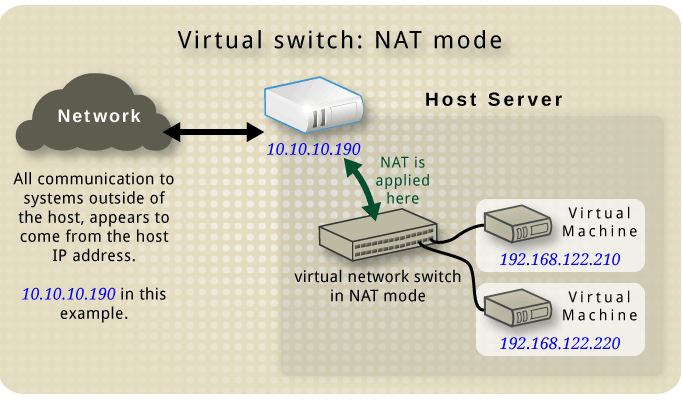
\includegraphics[scale=0.5]{Figures/Figure10.png}
	\caption[Virtual network on NAT mode]{Virtual network on NAT mode \cite{Reference19}}
	\label{fig:Virtual network on NAT mode}
\end{figure}


\section{KVM installation}
KVM is a virtualization feature in the Linux kernel that lets a program like qemu safely execute guest code directly on the host CPU. 
This is only possible when the target architecture is supported by the host CPU. 
CPU’s virtualization extension (VMX for Intel’s processors and SVM for AMD.) support could be verified by issuing this following command in a terminal:
\shellcmd{ grep -c '(vmx|svm)' /proc/cpuinfo }
A return value greater than zero means that current CPU supports KVM. In addition, it’s necessary to check virtualization technology is enabled in BIOS. 
After enabling this feature, we have to cold power-cycle the machine for the change to take effect. 
Once this is done, run kvm-ok to verify:  
\begin{figure}[htbp]
	\centering
		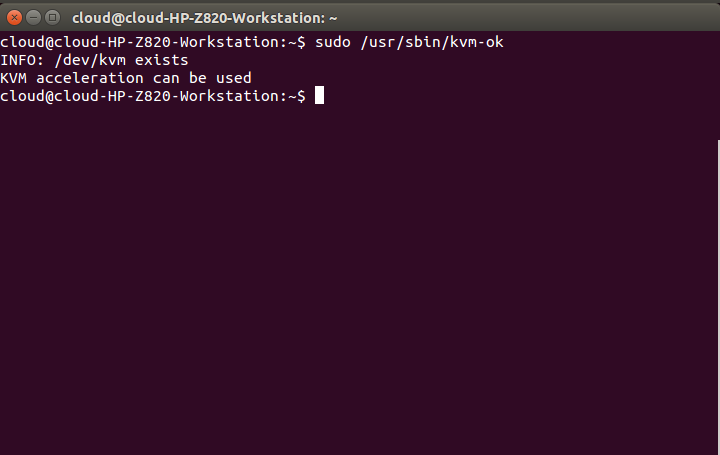
\includegraphics[scale=0.7]{Figures/Figure11.png}
	\caption[Output of kvm-ok command]{Output of kvm-ok command}
	\label{fig:Output of kvm-ok command}
\end{figure}

Then we begin to install required packages for KVM. The command to install everything you need is:
\shellcmd{ sudo apt-get install qemu-kvm libvirt-bin ubuntu-vm-builder bridge-utils}
\shellcmd{ sudo apt-get install virt-manager virtinst qemu-system}
Out of interest, KVM doesn’t have its own configuration directory. The configuration files could be found in: /etc/libvirt/qemu/
There are some quirks or confusions which deserve clarify, in term of difference and association between libvirt, 
qemu, qemu-kvm. Qemu in fact is project independent of KVM, it is an emulator which itself could be used as a virtualization 
alternative. Qemu-kvm is fork of QEMU maintained by KVM project. Currently (close to the 1.1 release) it still provides the best 
performance and certain additional features for using KVM with QEMU on x86. Any other architecture is already fully supported by QEMU itself. However QEMU development community plans to suspend the development of qemu-kvm and make qemu master fork to support all architectures. Libvirt is a toolkit to interact with the virtualization capabilities of recent versions of Linux [23]. It is an open-source project and provides a set of long term stable C API. These C APIs all APIs are designed to do virtualization management, such as: provision, create, modify, monitor, control, migrate and stop the guests - within the limits of the support of the hypervisor for those operations. Hence, libvirt is intended to be a building block for higher level management tools and for applications focusing on virtualization of a single physical host. The following picture shows the relationship between hypervisor, libvirt and virtualization management tool. 

\section{KVM Win7 Guest Manipulation} 
After establishing KVM virtualization platform, we plan to create a Windows 7 64 bits guest with virt-manager. 
To launch virt-manager, open a terminal and issue the following command: 
\shellcmd{ sudo virt-manager}
We name this guest as ``win7\_64bit'', chose a local installation place then click forward button.
\begin{figure}[htbp]
	\centering
		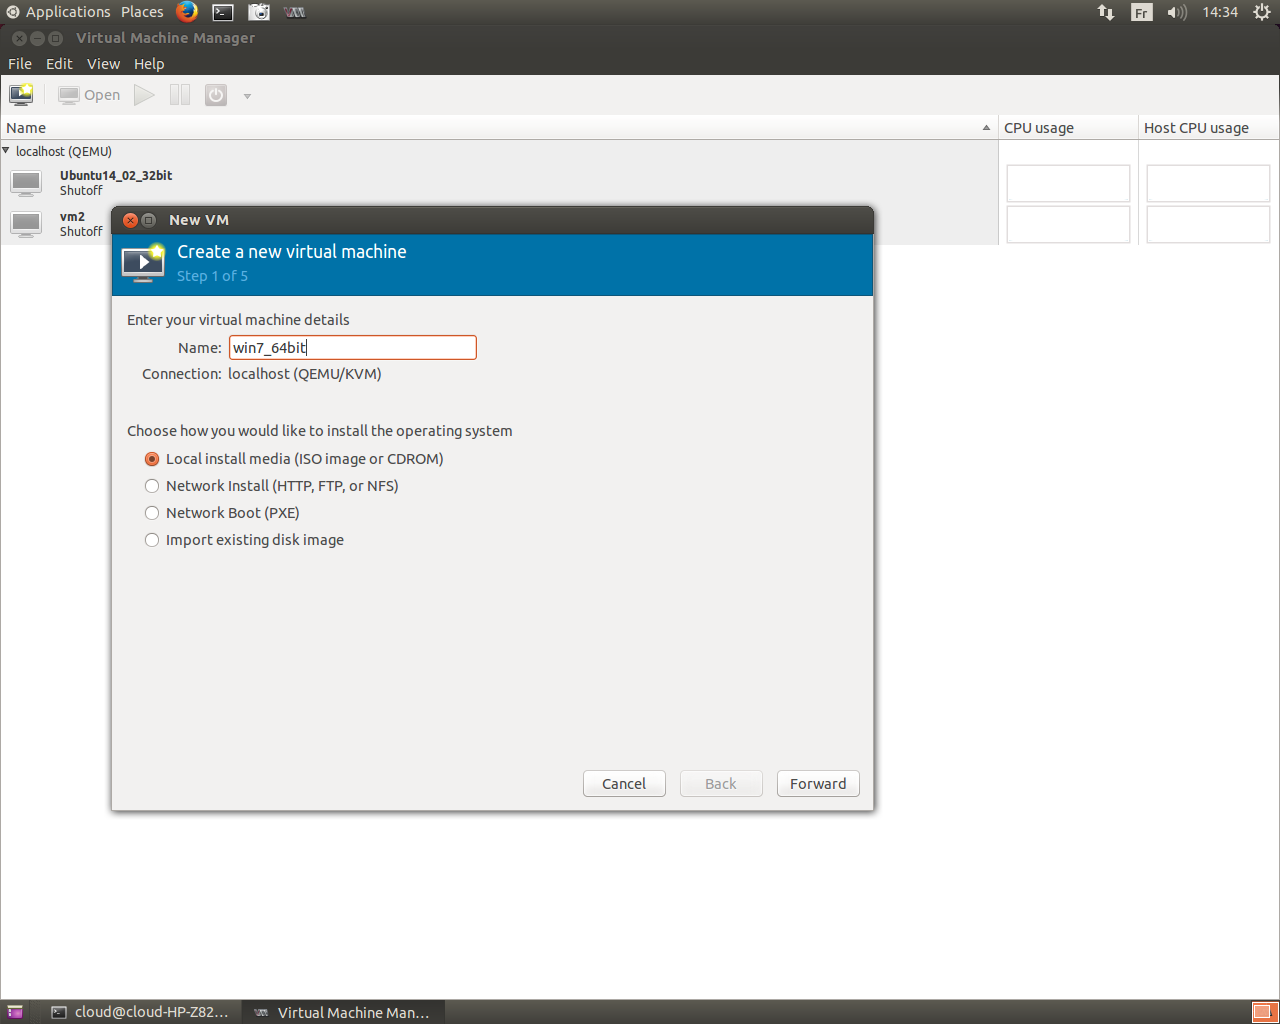
\includegraphics[scale=0.4]{Figures/Figure12.png}
	\caption[Step 1-Create a new VM with name win7\_64bit]{Step 1-Create a new VM with name win7\_64bit}
	\label{fig:Step 1-Create a new VM with name win7-64bit}
\end{figure}

At step 2 shown in Figure \ref{fig:Choose win7 ISO file}, we need to indicate the location of the win7 installation ISO file for virt-manager.
\begin{figure}[htbp]
	\centering
		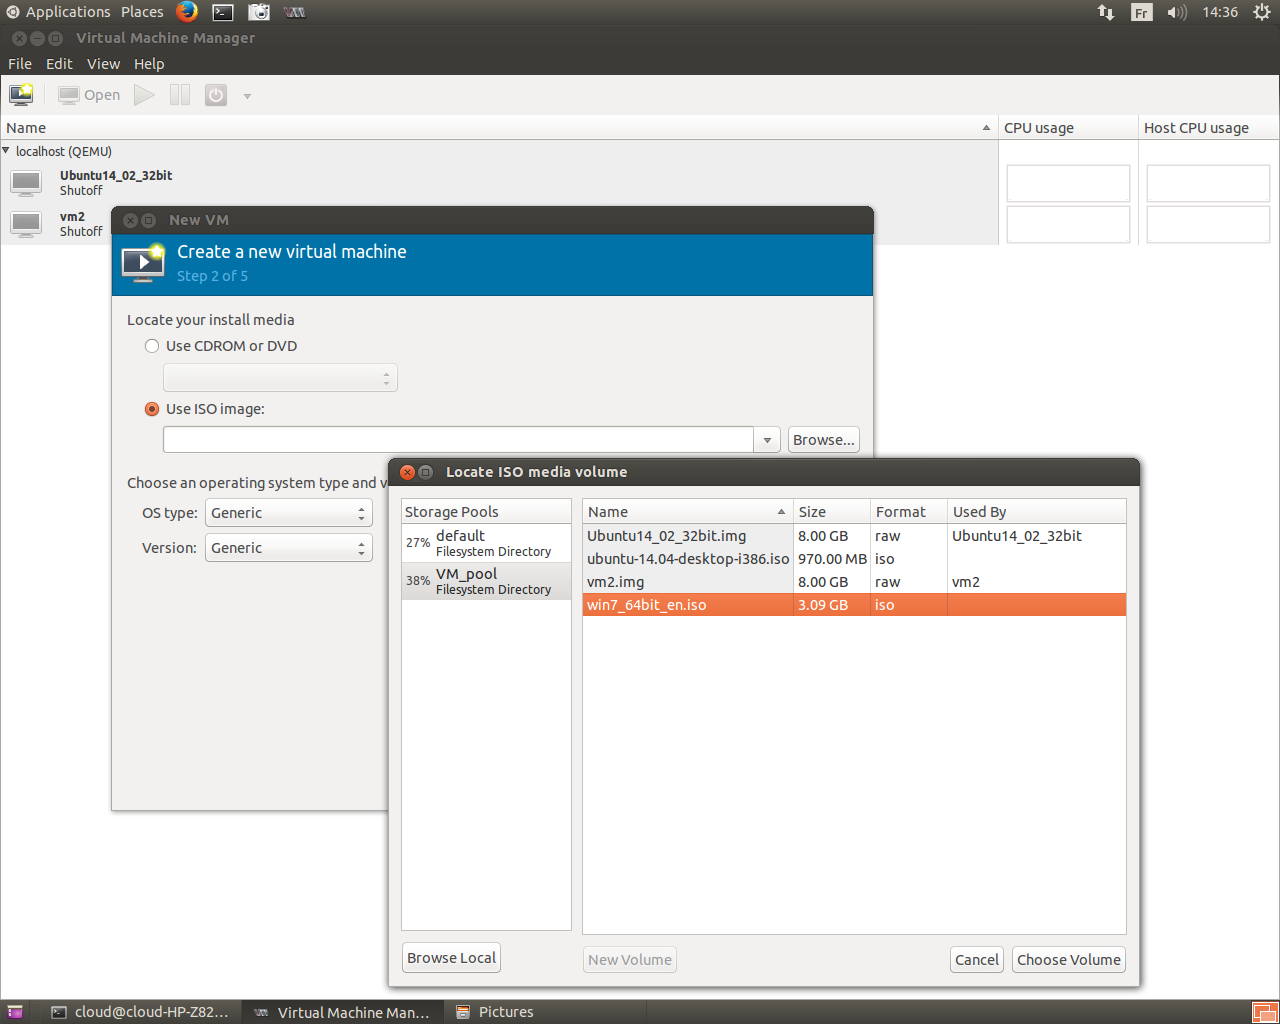
\includegraphics[scale=0.4]{Figures/Figure13.png}
	\caption[Step 2-Choose win7 ISO file]{Step 2-Choose win7 ISO file}
	\label{fig:Choose win7 ISO file}
\end{figure}

Then we create a virtual disk of 20G for our guest in step 3 (Figure \ref{fig:Step 3-Create a virtual disk of 20G}).
\begin{figure}[htbp]
	\centering
		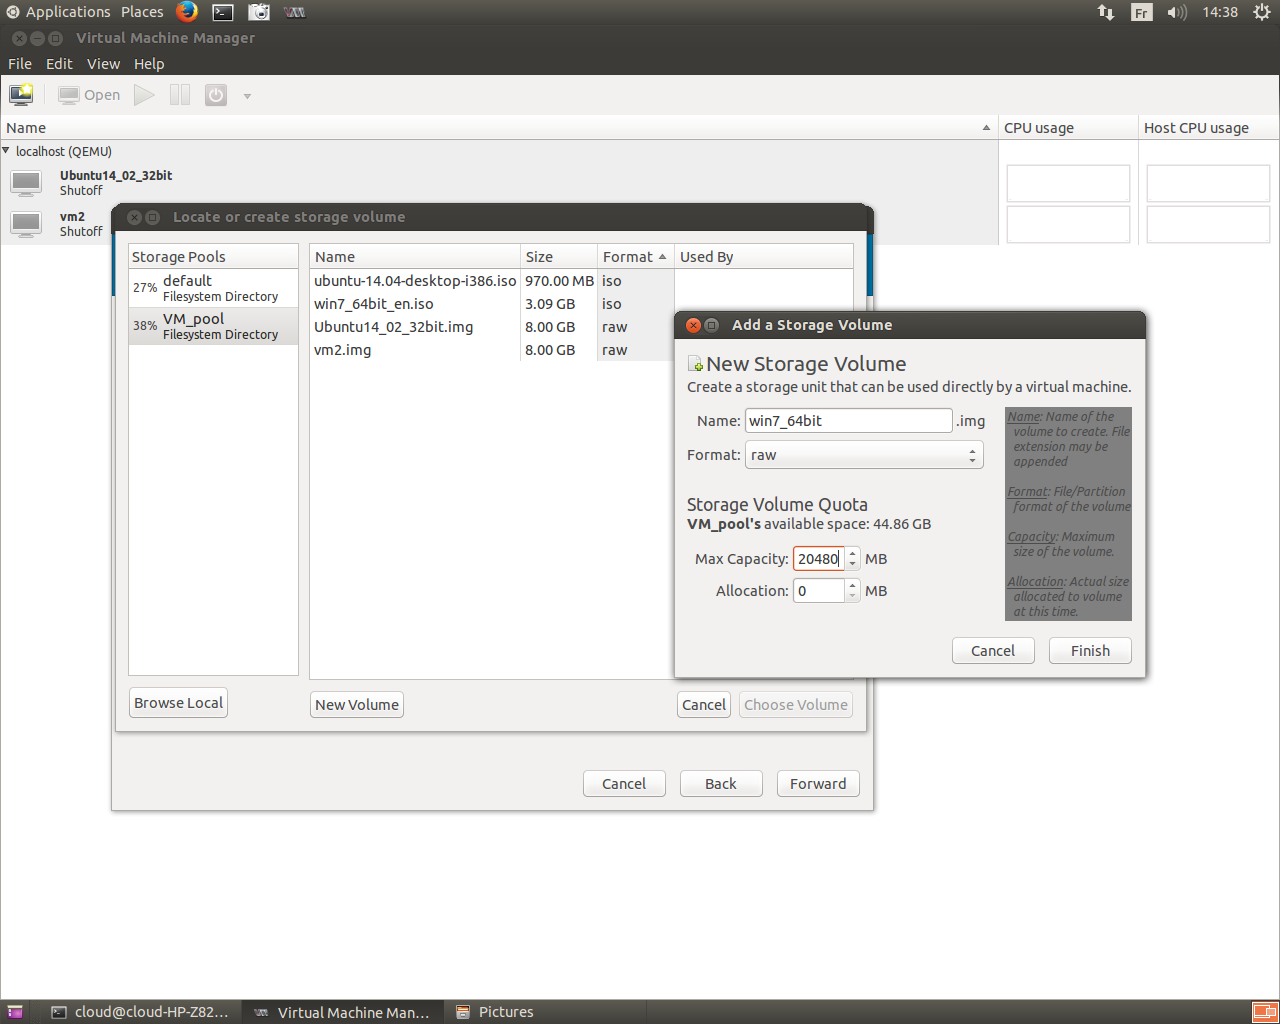
\includegraphics[scale=0.4]{Figures/Figure14.png}
	\caption[Step 3-Create a virtual disk of 20G]{Step 3-Create a virtual disk of 20G}
	\label{fig:Step 3-Create a virtual disk of 20G}
\end{figure}

In the next step (Figure \ref{fig:Step 4-Indicate virtual disk location for guest installation}), our reserved virtual disk is used as hard disk for win7\_64bit guest.
\begin{figure}[htbp]
	\centering
		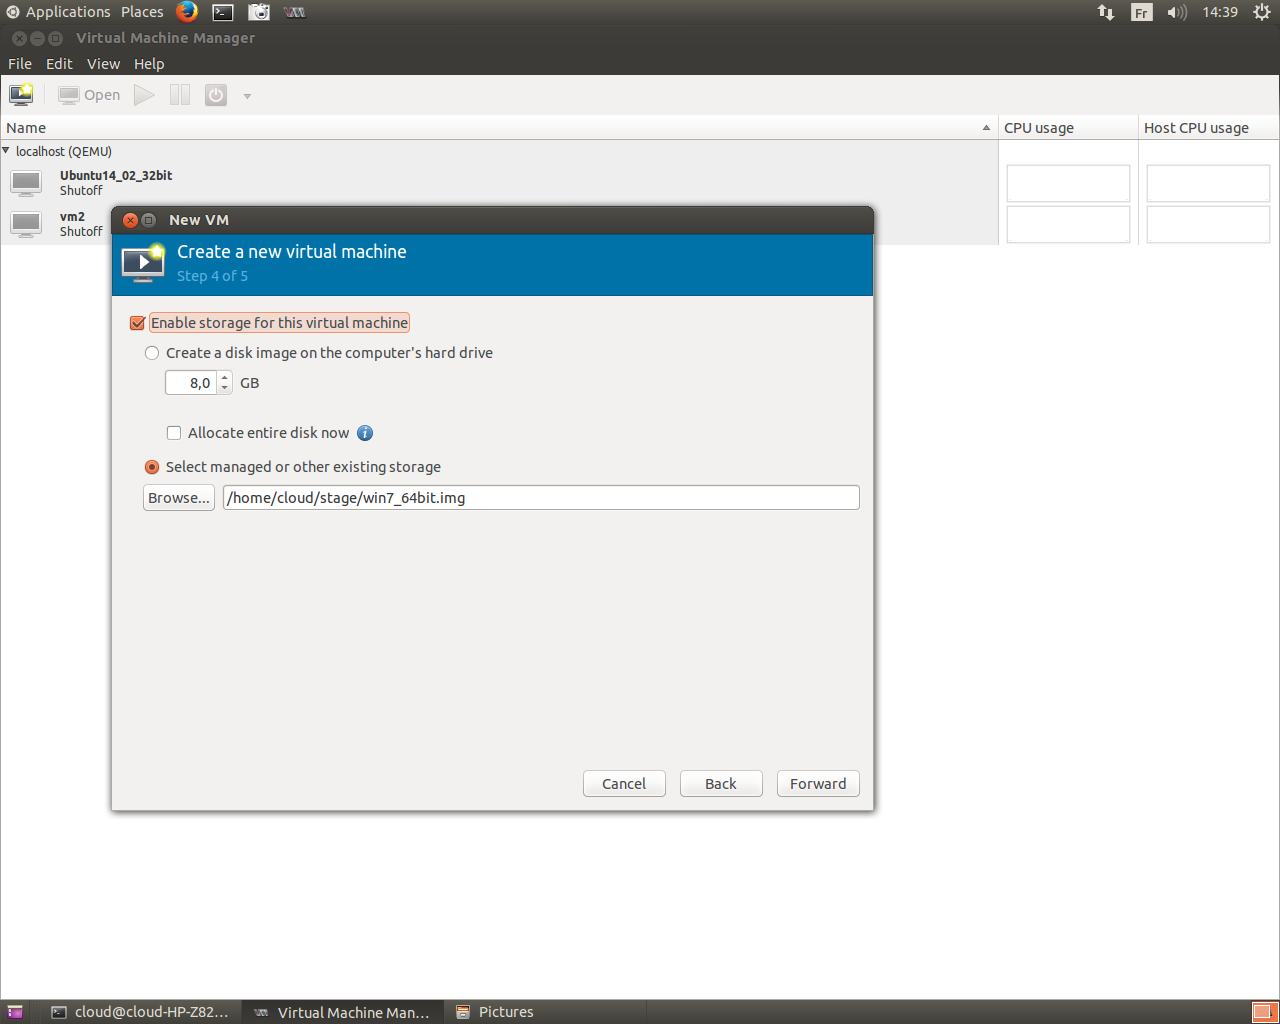
\includegraphics[scale=0.4]{Figures/Figure15.png}
	\caption[Step 4-Indicate virtual disk location for guest installation]{Step 4-Indicate virtual disk location for guest installation}
	\label{fig:Step 4-Indicate virtual disk location for guest installation}
\end{figure}

The last step (Figure \ref {fig:Step 5-Guest installation configuration resume}) is a resume of installation configuration. Note that the guest works with NAT network mode.
\begin{figure}[htbp]
	\centering
		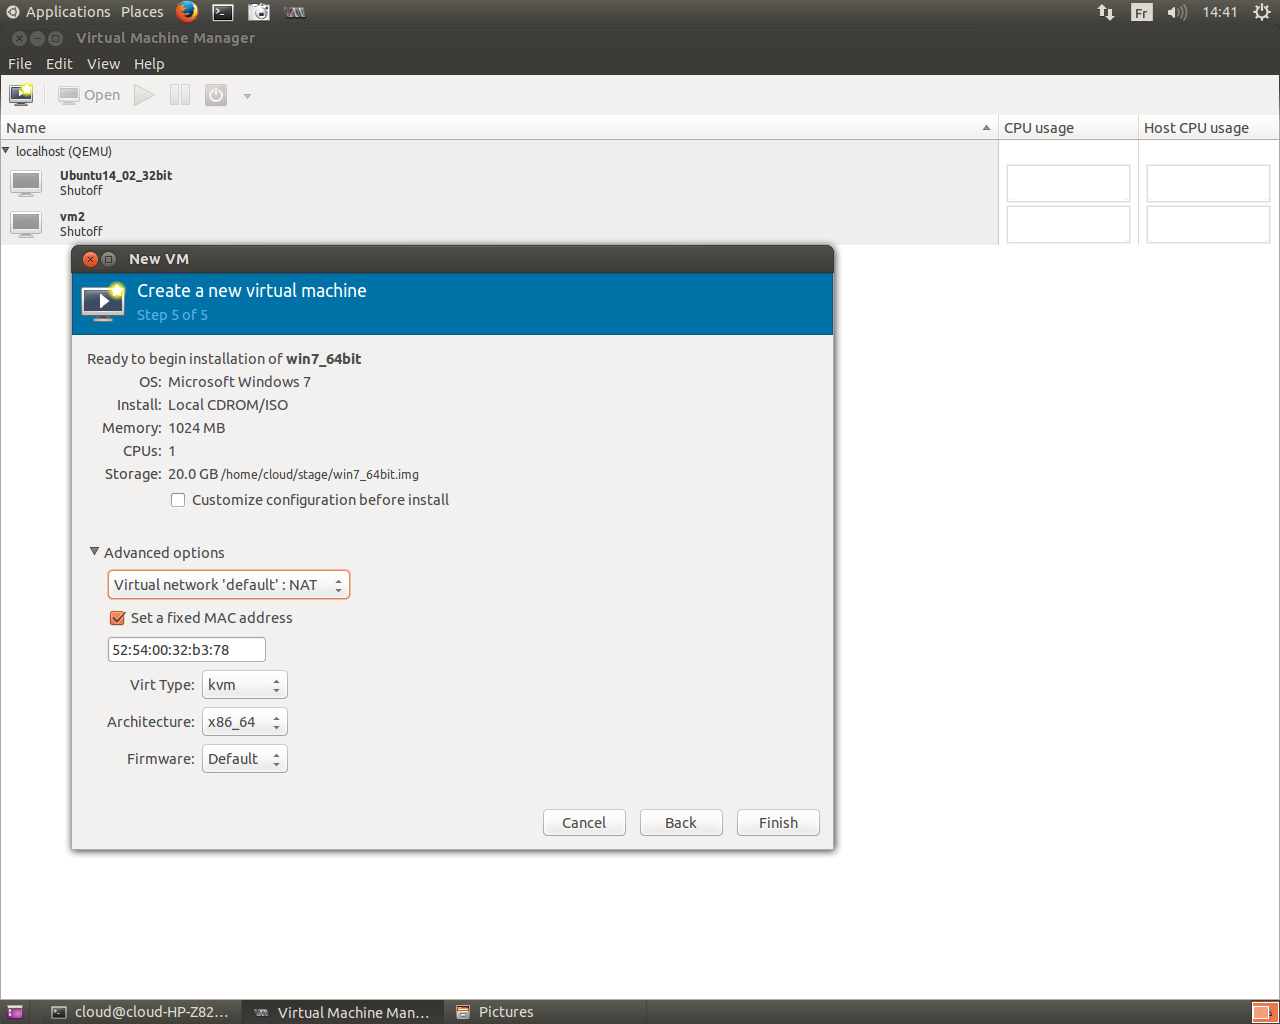
\includegraphics[scale=0.4]{Figures/Figure16.png}
	\caption[Step 5-Guest installation configuration resume]{Step 5-Guest installation configuration resume}
	\label{fig:Step 5-Guest installation configuration resume}
\end{figure}

When the installation process is finished, we check guest’s IP configuration and ping the host. The result is shown in picture \ref{fig:guest machine ping host machine}.
\begin{figure}[htbp]
	\centering
		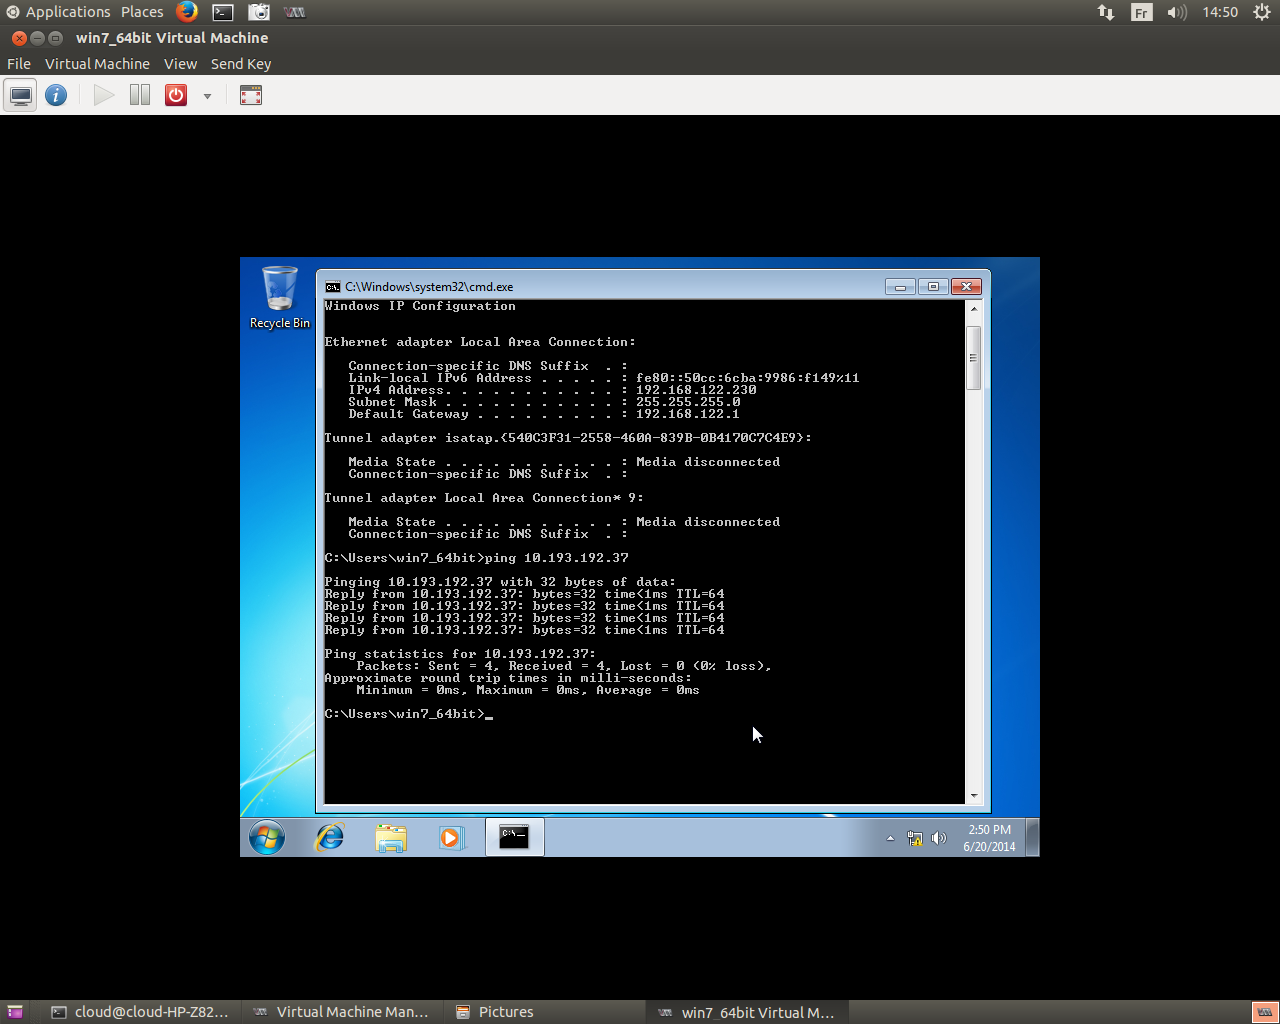
\includegraphics[scale=0.4]{Figures/Figure17.png}
	\caption[Guest machine ping host machine]{Guest machine ping host machine}
	\label{fig:guest machine ping host machine}
\end{figure}

Then verify that the guest machine is launched as a seperate process under Ubuntu by qemu in host machine. The result is shown in Figure \ref{fig:Guest as a qemu process in host machine}
\begin{figure}[htbp]
	\centering
		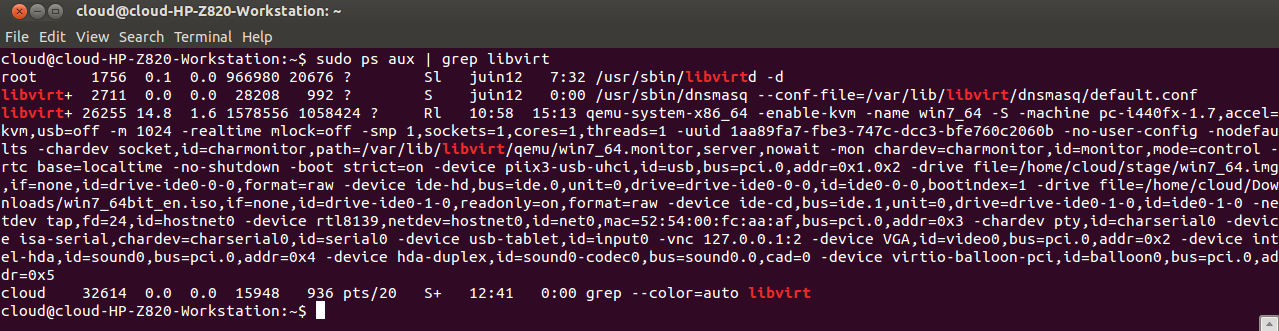
\includegraphics[width=14cm, height= 4cm ]{Figures/Figure18.png}
	\caption[Guest as a qemu process in host machine]{Guest as a qemu process in host machine}
	\label{fig:Guest as a qemu process in host machine}
\end{figure}


